\chapter{Taylor series integration} %Last updated 18-05-2016
\label{ch:tsi}

\section{General theory}
\label{sec:genTsiTheory}

\subsection{Workings of \ac{TSI}}
\label{subsec:workTsi}

\subsection{Step-size}
\label{subsec:stepSizeTsi}

\section{Associated equations}
\label{sec:assEq}
In order for \ac{TSI} to be implemented, the state derivatives have to be modelled as a set of continuous functions which are a function of the state only. This can be done in different ways. In this case, three cases were tested: two Cartesian cases and one spherical case. For the Cartesian cases, the initial conditions first have to be transformed into Cartesian coordinates. The Cartesian equations themselves require reference frame transformations, which can be written in two different ways. Both cases are described in \Cref{subsec:careq}. The reason for testing the spherical case is that the initial conditions are provided in spherical coordinates and the intermediate computations can be easily interpreted and checked for errors. However, the equations are highly sensitive to singularities. The spherical equations are described in \Cref{subsec:sphereq} and already include reference frame transformations. 

\subsection{Cartesian equations}
\label{subsec:careq}
The Cartesian state is described in \Cref{eq:state}, where $m_{MAV}$ is the mass of the \ac{MAV} and the subscript $I$ refers to the inertial frame.

\begin{align} \label{eq:state}
\mathbf{r}&=\begin{pmatrix}
x_{I}\\
y_{I}\\
z_{I}\\
\end{pmatrix}
&
\mathbf{V}&=\begin{pmatrix}
V_{x_{I}} \\
V_{y_{I}} \\
V_{z_{I}}\\
\end{pmatrix}
&
m_{MAV}&
\end{align}

The corresponding state derivatives are then described by \Cref{eq:state_derivatives}.

\begin{align} \label{eq:state_derivatives}
\begin{split} 
\dot{x}_{I}&=V_{x_{I}}\\
\dot{y}_{I}&=V_{y_{I}}\\
\dot{z}_{I}&=V_{z_{I}}
\end{split} 
&
\begin{split}
\ddot{x}_{I}&=\dot{V}_{x_{I}}=a_{x_{I}}\\
\ddot{y}_{I}&=\dot{V}_{y_{I}}=a_{y_{I}}\\
\ddot{z}_{I}&=\dot{V}_{z_{I}}=a_{z_{I}}
\end{split}
&
\dot{m}_{MAV}=-\dfrac{T}{g_{0}I_{sp}}
\end{align}

From this point on, the subscript $I$ is omitted, because the state and the state derivatives are always presented in the inertial frame. If variables have to be presented in any other reference frame the corresponding subscripts will be provided and explained. The accelerations in the x-, y- and z-direction have three contributing components: gravitational acceleration, drag and thrust. The gravitational acceleration can be directly expressed in the inertial frame, however the drag is presented in the body frame and the thrust is expressed in the propulsion frame. Therefore, both the drag and thrust contributions have to be transformed to the inertial frame using transformation matrices. This then results in the expression for the acceleration vector as shown by \Cref{eq:acc}. The subscript $G$ shows that the parameter is a function of the ground velocity.

\begin{multline} \label{eq:acc}
\begin{pmatrix}
a_{x}\\
a_{y}\\
a_{z}\\
\end{pmatrix}
=
\begin{pmatrix}
-\mu_{M}\dfrac{x}{r^{3}}\\
-\mu_{M}\dfrac{y}{r^{3}}\\
-\mu_{M}\dfrac{z}{r^{3}}\\
\end{pmatrix}+
\Bigg|_{\mathbf{I}}\mathbb{T}_{\mathbf{z}}\left(-\Omega_{M}t_{O}+\omega_{P}\right)\Bigg|_{\mathbf{R}}\mathbb{T}_{\mathbf{z}}\left(-\tau\right)\mathbb{T}_{\mathbf{y}}\left(\dfrac{\pi}{2}+\delta\right)\Bigg|_{\mathbf{V}}\mathbb{T}_{\mathbf{z}}\left(-\chi_{G}\right)\mathbb{T}_{\mathbf{y}}\left(-\gamma_{G}\right)\Bigg|_{\mathbf{B}}\left[
\begin{pmatrix}
-\dfrac{D}{m_{MAV}}\\
0\\
0\\
\end{pmatrix}
+  \right. \dots \\
\dotsc
 \left.
\Bigg|_{\mathbf{B}}\mathbb{T}_{\mathbf{z}}\left(-\psi_{T}\right)\mathbb{T}_{\mathbf{y}}\left(-\epsilon_{T}\right)\Bigg|_{\mathbf{P}}
\begin{pmatrix}
\dfrac{T}{m_{MAV}}\\
0\\
0\\
\end{pmatrix}
\right]
\end{multline}

It can be seen that this set of equations is a function of the current position and many other parameters. These parameters will all have to be written as a function of the current state. This can be done by writing them into auxiliary equations, forming extra variables that then also require the auxiliary derivatives. This works for certain parameters, such as the gravity, because these equations are already expressed in the inertial frame. However, the transformation angles are defined in different reference frames, which means that finding the proper auxiliary derivatives can be tricky sometimes. Therefore it was decided to directly write these parameters as auxiliary functions. Each of the auxiliary functions performs one simple algebraic operation and the collection of these auxiliary functions then form the complete set of recurrence relations using the recurrence relations for the simple algebraic operations. This is all described in \Cref{subsec:recRelAuxFunc}. 

For the auxiliary equations, a similar notation will be used as shown by \cite{scott2008high}. Here the equations are denoted by $x_{number}$ and the corresponding derivatives $x'_{number}$. This notation will also be used for the current state and the corresponding state derivatives. This way, \Cref{eq:state} can be written as \Cref{eq:stateX} and the corresponding derivatives can be written as presented by \Cref{eq:state_derivativesX}.

\begin{align} \label{eq:stateX}
\begin{split} 
x_{1}&=x\\
x_{2}&=y\\
x_{3}&=z
\end{split} 
&
\begin{split}
x_{4}&=\dot{x}=V_{x}\\
x_{5}&=\dot{y}=V_{y}\\
x_{6}&=\dot{z}=V_{z}
\end{split}
&
x_{7}=m_{MAV}
\end{align}


\begin{align} \label{eq:state_derivativesX}
\begin{split} 
x'_{1}&=x_{4}\\
x'_{2}&=x_{5}\\
x'_{3}&=x_{6}
\end{split} 
&
\begin{split}
x'_{4}&=\dot{V}_{x}=a_{x}=a_{g,x}+a_{D,x}+a_{T,x}\\
x'_{5}&=\dot{V}_{y}=a_{y}=a_{g,y}+a_{D,y}+a_{T,y}\\
x'_{6}&=\dot{V}_{z}=a_{z}=a_{g,z}+a_{D,z}+a_{T,z}
\end{split}
&
x'_{7}=\dot{m}_{MAV}=-\dfrac{T}{g_{0}I_{sp}}
\end{align}

In this case the thrust and specific impulse are constant, which means that $x'_{7}$ is constant and any additional derivative will be zero. Also, neither one of the thrust angles is a function of the state, which means that $a_{T}$, in the body frame, is only a function of $x_{7}$ (also see \Cref{eq:acc}). However, both $a_{g}$ and $a_{D}$ are a function of the position and velocity, where $a_{D}$ is also a function of the \ac{MAV} mass. Only $a_{g}$ is rewritten using auxiliary equations as mentioned before. This is shown in \Cref{subsubsec:tsiGravity}.


%For the numbering of all the auxiliary equations goes that the order comes from the manner in which they were all written out on paper. This means that sometimes higher number parameters could contain much lower number parameters without the intermediate parameters defined yet. However, these will all be defined eventually.


\subsubsection{Gravitational acceleration}
 \label{subsubsec:tsiGravity} 
 For the gravitational acceleration two auxiliary equations were required since $r=\sqrt{x^{2}+y^{2}+z^{2}}$. The resulting expressions for the gravitational acceleration are shown in \Cref{eq:gravAcc} with the corresponding auxiliary equations and the derivatives defined in \Cref{eq:gravAux}.
 
 \begin{equation} \label{eq:gravAcc}
\begin{split}
a_{g,x} &= -\mu_{M}\dfrac{x_{1}}{r^{3}} = \dfrac{x_{1}}{\left(x_{1}^{2}+x_{2}^{2}+x_{3}^{2} \right)^{3/2}}=-\mu_{M}\dfrac{x_{1}}{x_{9}}\\
a_{g,y} &= -\mu_{M}\dfrac{x_{2}}{r^{3}} = \dfrac{x_{2}}{\left(x_{1}^{2}+x_{2}^{2}+x_{3}^{2} \right)^{3/2}}=-\mu_{M}\dfrac{x_{2}}{x_{9}}\\
a_{g,z} &= -\mu_{M}\dfrac{x_{3}}{r^{3}} = \dfrac{x_{3}}{\left(x_{1}^{2}+x_{2}^{2}+x_{3}^{2} \right)^{3/2}}=-\mu_{M}\dfrac{x_{3}}{x_{9}}
\end{split}
\end{equation}

\begin{align} \label{eq:gravAux}
\begin{split} 
x_{8}&=x_{1}^{2}+x_{2}^{2}+x_{3}^{2}\\
x_{9}&=x_{8}^{3/2}
\end{split} 
&
\begin{split}
x'_{8}&=2x_{1}x_{4}+2x_{2}x_{5}+2x_{3}x_{6}\\
x'_{9}&=\dfrac{3}{2}\dfrac{x_{9}x_{8}'}{x_{8}}
\end{split}
\end{align}
 
 
 
\subsubsection{Transformation angles}
\label{subsubsec:tsiTransAngl}
The angles required for the transformation to go from the body frame to the reference frame all have to be written as a function of the state variables. The required angles are $\lambda$, $\delta$, $\chi_{G}$ and $\gamma_{G}$. Here $\lambda = \tau + \Omega_{M}t_{O}-\omega_{P}$. This means that instead of first transforming to the rotating frame completely and then transforming to the inertial frame, an inertial longitude angle $\lambda$ can be defined to directly transform to the inertial frame. The first two angles are the longitude and latitude and are spherical coordinates. Thus the relations for these angles can be found using the transformation from the Cartesian to the spherical system. However, the angles themselves are not required directly, because they are only used in transformation matrices. These matrices are comprised of the sines and cosines of these angles, which means that a direct relation between the state variables and the sines and cosines of the position angles can be used. These relations can be derived from \Cref{fig:sphertocart_noomen2013basic} and are described in \Cref{eq:transAngl}


 \begin{figure}[!ht]
\centering
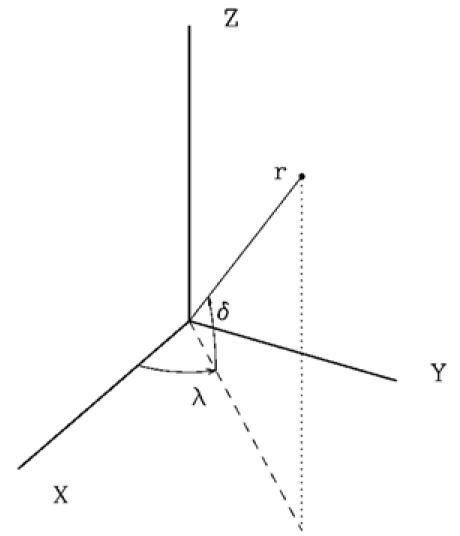
\includegraphics[width=0.7\textwidth]{figures/reference_frames/sphertocart_noomen2013basic.jpg}
\caption{Spherical position variables in an inertial Cartesian frame \citep{noomen2013basic}.}
\label{fig:sphertocart_noomen2013basic}
\end{figure}

\begin{align} \label{eq:transAngl}
\begin{split}
r = \sqrt{x^{2}+y^{2}+z^{2}}\\
\end{split}
&
\begin{split}
\sin \lambda &= \dfrac{y}{\sqrt{x^{2}+y^{2}}}\\
\cos \lambda &= \dfrac{x}{\sqrt{x^{2}+y^{2}}}\\
\end{split}
&
\begin{split}
\sin \delta &= \dfrac{z}{r}\\
\cos \delta &= \dfrac{\sqrt{x^{2}+y^{2}}}{r}
\end{split} 
\end{align} 

The corresponding auxiliary functions can then be described by \Cref{eq:auxFtransAngl} using the definitions provided in \Cref{eq:stateX,eq:state_derivativesX}.

\begin{align} \label{eq:AuxFtransAngl}
\begin{split}
w_{4,1} &= x_{1}^{2}+x_{2}^{2} \\
w_{4,2} &= w_{4,1}+x_{3}^{2} \\
w_{4,3} &= r = \sqrt{w_{4,2}} \\
w_{4,4} &= \sqrt{w_{4,1}} \\
\end{split}
&
\begin{split}
w_{4,5} &= s\lambda = \dfrac{x_{2}}{w_{4,4}}\\
w_{4,6} &= c\lambda = \dfrac{x_{1}}{w_{4,4}} \\
\end{split}
&
\begin{split}
w_{4,7} &= s\delta = \dfrac{x_{3}}{w_{4,3}} \\
w_{4,8} &= c\delta = \dfrac{w_{4,4}}{w_{4,3}}\\
\end{split} 
\end{align} 


The latitude and longitude could be described using the position vector in the inertial frame, however the transformation from the body frame to the vertical frame is a function of the ground (underscore 'G') velocity in the rotational frame. Since the position and velocity in the inertial frame are known (current state), the ground velocity ($V_{G}$) can be written as a function of the inertial velocity ($V_{I}$). For this, the velocity components have to be transformed from the inertial frame to the vertical frame (which is the inverse of the first three transformations described in \Cref{eq:acc}). This transformation is shown in \Cref{eq:VItoVV} and was described in \cite{mooij1994motion}. Here, $c$ stands for cosine and $s$ stands for sine. This transformation also includes the rotational effect on the velocity due to the rotation of Mars.
 
 \begin{equation} \label{eq:VItoVV}
\mathbf{V_{V}} =  
 \begin{pmatrix}
V_{x_{V}}\\
V_{y_{V}}\\
V_{z_{V}}\\
\end{pmatrix}
=
\left[
\begin{matrix}
-c\lambda s\delta & -s\lambda s\delta & c\delta\\
-s\lambda & c\lambda & 0\\
-c\lambda c\delta & -s\lambda c\delta & -s\delta\\
\end{matrix}
\right]
\left\lbrace
\begin{pmatrix}
V_{x}\\
V_{y}\\
V_{z}\\
\end{pmatrix}
-
\begin{pmatrix}
0 \\
0 \\
\Omega_{M} \\
\end{pmatrix}
\times
\begin{pmatrix}
x \\
y \\
z \\
\end{pmatrix}
\right\rbrace
 \end{equation}
 
The ground velocity can now be computed as the norm of the vertical velocity vector as shown by \Cref{eq:VG}. The transformation matrices disappear because the norm of a transformation matrix is simply 1, which means that $V_{G}=V_{V}=V_{R}$.

\begin{equation} \label{eq:VG}
V_{G} = \| \mathbf{V_{V}} \| = 
\left\Vert
\begin{pmatrix}
V_{x}\\
V_{y}\\
V_{z}\\
\end{pmatrix}
-
\begin{pmatrix}
0 \\
0 \\
\Omega_{M} \\
\end{pmatrix}
\times
\begin{pmatrix}
x \\
y \\
z \\
\end{pmatrix}
\right\Vert 
\end{equation}

\Cref{eq:VG} can be rewritten as \Cref{eq:xfifteen}.

\begin{equation}\label{eq:xfifteen}
V_{G} = \sqrt{\left(V_{x}+\Omega_{M}y\right)^{2}+\left(V_{y}-\Omega_{M}x\right)^{2}+V_{z}^{2}} 
\end{equation}

The corresponding auxiliary functions are provided in \Cref{eq:velocityAuxF}.

\begin{align} \label{eq:velocityAuxF}
\begin{split}
w_{4,9} &= V_{x}+\Omega_{M}y \\
w_{4,10} &= V_{y}-\Omega_{M}x \\
\end{split}
&
\begin{split}
w_{4,11} &= w_{4,9}^{2}+w_{4,10}^{2}+x_{6}^{2} \\
w_{4,12} &= V_{G}=\sqrt{w_{4,11}} \\
\end{split} 
\end{align} 

%\sqrt{V_{I}^{2}+\Omega_{M}^{2}\left(x^{2}+y^{2}\right)+2\Omega_{M}\left(V_{x}y-V_{y}x\right)} \quad \text{where} \quad V_{I}=\sqrt{V_{x}^{2}+V_{y}^{2}+V_{z}^{2}} \\
 
The spherical velocity angles can now be derifed from \Cref{fig:vertical_spherical_mooij1994motion} as described by \Cref{eq:velAngl}. These were also provided by \cite{mooij1994motion}. 

 \begin{figure}[!ht]
\centering
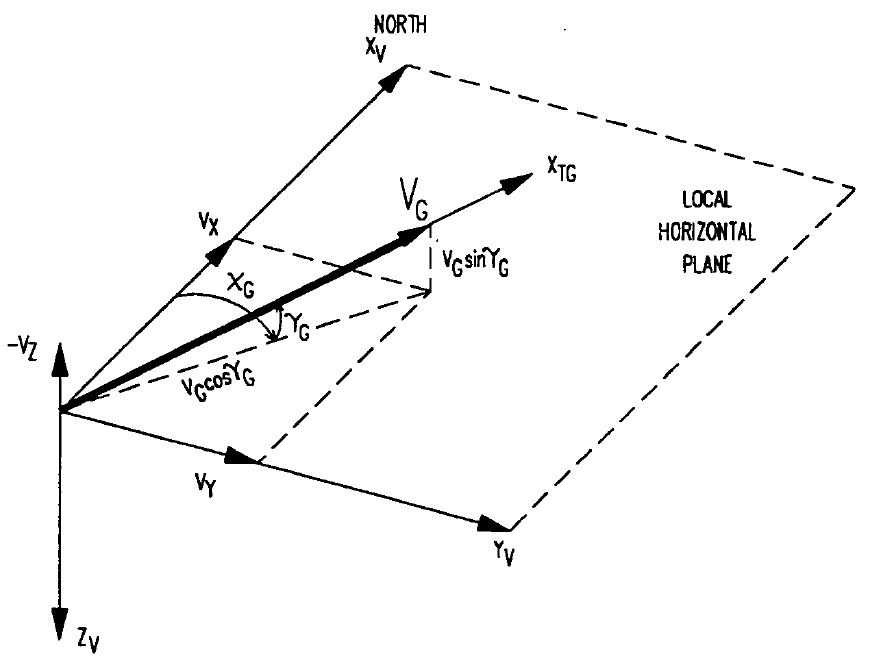
\includegraphics[width=0.7\textwidth]{figures/reference_frames/vertical_spherical_mooij1994motion.jpg}
\caption{Spherical velocity variables in a vertical Cartesian frame \citep{mooij1994motion}.}
\label{fig:vertical_spherical_mooij1994motion}
\end{figure}



\begin{align} \label{eq:velAngl}
\begin{split}
\sin \chi_{G} &= \dfrac{V_{y_{V}}}{\sqrt{V_{x_{V}}^{2}+V_{y_{V}}^{2}}} \\
\cos \chi_{G} &= \dfrac{V_{x_{V}}}{\sqrt{V_{x_{V}}^{2}+V_{y_{V}}^{2}}} \\
\end{split}
&
\begin{split}
\sin \gamma_{G} &= \dfrac{-V_{z_{V}}}{V_{G}}\\
\cos \gamma_{G} &= \dfrac{\sqrt{V_{x_{V}}^{2}+V_{y_{V}}^{2}}}{V_{G}}\\
\end{split} 
\end{align} 


Here, $V_{x_{V}}$, $V_{y_{V}}$ and $V_{z_{V}}$ are the velocities in the vertical frame. Expressions for these variables can be obtained by rewriting \Cref{eq:VItoVV}. This then results in \Cref{eq:VV}.


\begin{equation} \label{eq:VV}
\begin{split}
V_{x_{V}} & = -\left(V_{x}+\Omega_{M}y\right) s \delta c\lambda - \left(V_{y}-\Omega_{M}x\right) s\delta s\lambda+V_{z}c\delta \\
V_{y_{V}} & = \left(V_{y}-\Omega_{M}x\right) c\lambda - \left(V_{x}+\Omega_{M} y \right) s\lambda \\
V_{z_{V}} & = -\left(V_{x}+\Omega_{M}y\right)-\left(V_{y}-\Omega_{M}x\right) c\delta s\lambda - V_{z} s\delta \\
\end{split}
\end{equation}

The combined auxiliary functions for \Cref{eq:velAngl,eq:VV} are described in \Cref{eq:velocityAuxF}.

\begin{align} \label{eq:VV}
\begin{split}
w_{4,13} &= -c\lambda s\delta  = -w_{4,6}w_{4,7} \\
w_{4,14} &= -s\delta s\lambda = -w_{4,7}w_{4,5} \\
w_{4,15} &= -c\delta c\lambda = -w_{4,8}w_{4,6} \\
w_{4,16} &= -c\delta s\lambda = w_{4,8}w_{4,5} \\
\end{split}
&
\begin{split}
w_{4,17} &= V_{x_{V}} = x_{6}w_{4,8}+w_{4,9}w_{4,13}+w_{4,10}w_{4,14} \\
w_{4,18} &= V_{y_{V}} = w_{4,10}w_{4,6}-w_{4,9}w_{4,5} \\
w_{4,19} &= V_{z_{V}} = w_{4,9}w_{4,15}-x_{6}w_{4,7}+w_{4,10}w_{4,16} \\
w_{4,20} &= V_{x_{V}}^{2}+V_{y_{V}}^{2} = w_{4,17}^{2}+w_{4,18}^{2} \\
w_{4,21} &= \sqrt{w_{4,20}} \\
\end{split}
&
\begin{split}
w_{4,22} &= s\chi_{G} = \dfrac{w_{4,18}}{w_{4,21}} \\
w_{4,23} &= c\chi_{G} = \dfrac{w_{4,17}}{w_{4,21}} \\
w_{4,24} &= s\gamma_{G} = -\dfrac{w_{4,19}}{w_{4,12}} \\
w_{4,25} &= c\gamma_{G} = \dfrac{w_{4,21}}{w_{4,12}} \\
\end{split}
\end{align}



 \subsubsection{Drag acceleration}
 \label{subsubsec:tsiDrag}
The drag acceleration is determined in the body frame by dividing the drag force ($D$) by the mass of the \ac{MAV} ($x_{7}$). The drag force itself is a function of the position and velocity. The equations associated with the drag function are described in \Cref{eq:dragAux} and the corresponding derivatives are presented by \Cref{eq:dragDerAux} except for the $C_{D}$ equations. The polynomial coefficients for the density equation are provided in \Cref{tab:fitParametersDen} and are represented in \Cref{eq:dragAux} by $P_{\rho}$.

 \begin{equation} \label{eq:dragAux}
\begin{split}
h &= r-R_{MOLA} \\
D &= \frac{1}{2}\rho V_{G}^{2}SC_{D}\\
\rho &= e^{P_{\rho 10}h^{10}+P_{\rho 9}h^{9}+P_{\rho 8}h^{8}+P_{\rho 7}h^{7}+P_{\rho 6}h^{6}+P_{\rho 5}h^{5}+P_{\rho 4}h^{4}+P_{\rho 3}h^{3}+P_{\rho 2}h^{2}+P_{\rho 1}h+P_{\rho 0}} \\
\end{split}
\end{equation}

Since the drag coefficient is a function of Mach number as by \Cref{fig:dragcoeff_whitehead2004mars} and is not a continuous function, it has to be split into 6 different sections. Each section has a separate $C_{D}-M$ relation. Before these relations can be described, three additional expressions are required which are described in \Cref{eq:cdAux}.

 \begin{equation} \label{eq:cdAux}
\begin{split}
M &= \dfrac{V}{a} \\
a &= \sqrt{\gamma_{a}R_{a}^{*}T_{a}} \quad \text{where} \quad R_{a}^{*}=\dfrac{R_{a}}{M_{a}} \\
\end{split}
\end{equation}

The conditional relations shown in \Cref{eq:cdCond} describe the different equations that have to be used associated with the different sections of the drag coefficient plot. Here $P_{C_{D} number,section}$ are the polynomial fit coefficients as provided in \Cref{tab:dragCoeffPara}.

\begin{equation}\label{eq:cdCond}
C_{D}=\begin{cases}
0.2, & \text{for } 0\leq M < 0.5\\
P_{C_{D} 1,2}M+P_{C_{D} 0,2}, &  \text{for } 0.5\leq M < 1 \\
P_{C_{D} 1,3}M+P_{C_{D} 0,3}, &  \text{for } 1\leq M < 1.3 \\
P_{C_{D} 1,4}M+P_{C_{D} 0,4}, &  \text{for } 1.3\leq M < 2.5 \\
P_{C_{D} 1,5}M+P_{C_{D} 0,5}, &  \text{for } 2.5\leq M < 4 \\
0.3, &  \text{for } M \geq 4 
\end{cases}\\
\end{equation}

This only leaves the temperature $T_{a}$, which is a function of the altitude $h$ in km,\ac{MOLA}. But as described in \Cref{subsec:atmofuncfit}, this parameter is split into different sections as well. The equations per section for the temperature is provided in \Cref{eq:tempCondAux}. Here $P_{T number,section}$ are the polynomial fit coefficients as provided in \Cref{tab:fitParameters}.

\begin{equation}\label{eq:tempCondAux}
T_{a}=\begin{cases}
P_{T 1,1}h+P_{T 0,1}, & \text{for } -0.6 \leq h < 5.04  \\
P_{T 3,2}h^{3}+P_{T 2,2}h^{2}+P_{T 1,2}h+P_{T 0,2}, &  \text{for } 5.04 \leq h < 35.53   \\
P_{T 6,3}h^{6}+P_{T 5,3}h^{5}+P_{T 4,3}h^{4}+P_{T 3,3}h^{3}+ \dots \\
\qquad\ \ \dotsc +P_{T 2,3}h^{2}+P_{T 1,3}h+P_{T 0,3}, &  \text{for } 35.53 \leq h < 75.07   \\
P_{T 8,4}h^{8}+P_{T 7,4}h^{7}+P_{T 6,4}h^{6}+P_{T 5,4}h^{5} \\
\qquad\ \ +P_{T 4,4}h^{4}+P_{T 3,4}h^{3}+P_{T 2,4}h^{2}+P_{T 1,4}h+P_{T 0,4}, &  \text{for } 75.07 \leq h < 170.05   \\
136.5, &  \text{for }  h \geq 170.05   
\end{cases}
\end{equation}

For both the conditional parameters $C_{D}$ and $T_{a}$  the required section has to be determined before the evaluation of the equations.

 \textbf{\textcolor{red}{Rest still has to be rewritten!!}}

\subsubsection{Thrust acceleration}
\label{subsubsec:tsiDrag}

\subsection{Spherical equations}
\label{subsec:sphereq}
 
 \subsubsection{Drag acceleration}
 \label{subsubsec:tsiDrag}
The drag acceleration is determined in the body frame by dividing the drag force ($D$) by the mass of the \ac{MAV} ($x_{7}$). The drag force itself is a function of the position and velocity. The equations associated with the drag function are described in \Cref{eq:dragAux} and the corresponding derivatives are presented by \Cref{eq:dragDerAux} except for the $C_{D}$ equations. The polynomial coefficients for the density equation are provided in \Cref{tab:fitParametersDen} and are represented in \Cref{eq:dragAux} by $P_{\rho}$.

 \begin{equation} \label{eq:dragAux}
\begin{split}
h &= r-R_{MOLA} \\
D &= \frac{1}{2}\rho V_{G}^{2}SC_{D}\\
\rho &= e^{P_{\rho 10}h^{10}+P_{\rho 9}h^{9}+P_{\rho 8}h^{8}+P_{\rho 7}h^{7}+P_{\rho 6}h^{6}+P_{\rho 5}h^{5}+P_{\rho 4}h^{4}+P_{\rho 3}h^{3}+P_{\rho 2}h^{2}+P_{\rho 1}h+P_{\rho 0}} \\
\end{split}
\end{equation}

 \begin{equation} \label{eq:dragDerAux}
\begin{split}
x'_{27} &= \frac{1}{2}Sx_{15}\left(x_{15} \left(x_{29}x'_{28}+x_{28}x'_{29}\right)+2x_{28}x_{29}x'_{15}\right) \\
x'_{28} &= x'_{30}x_{28} \\
x'_{30} &=x'_{31} \left(10 P_{\rho 10}x_{31}^{9}+9 P_{\rho 9}x_{31}^{8}+8 P_{\rho 8}x_{31}^{7}+7 P_{\rho 7}x_{31}^{6}+6 P_{\rho 6}x_{31}^{5}+\dots \right. \\
&  \left. \dotsc +5 P_{\rho 5}x_{31}^{4}+4 P_{\rho 4}x_{31}^{3}+3 P_{\rho 3}x_{31}^{2}+2 P_{\rho 2}x_{31}+P_{\rho 1}\right) \\
x'_{31} &= x'_{16}
\end{split}
\end{equation}

Since the drag coefficient is a function of Mach number as by \Cref{fig:dragcoeff_whitehead2004mars} and is not a continuous function, it had to be split into 6 different sections. Each section has a separate $C_{D}-M$ relation. Before these relations can be described, three additional auxiliary equations/expressions are required which are described in \Cref{eq:cdAux}.

 \begin{equation} \label{eq:cdAux}
\begin{split}
x_{32} &= M = \dfrac{V}{a} = \dfrac{x_{15}}{x_{33}}\\
x_{33} &= a = \sqrt{\gamma_{a}R_{a}^{*}T_{a}} = \sqrt{\gamma_{a}R_{a}^{*}x_{34}} \quad \text{where} \quad R_{a}^{*}=\dfrac{R_{a}}{M_{a}} \\
x_{34} &= T_{a}
\end{split}
\end{equation}

The conditional relations shown in \Cref{eq:cdCond} describe the different auxiliary equations that have to be used associated with the different sections. Here $P_{C_{D} number,section}$ are the polynomial fit coefficients as provided in \Cref{tab:dragCoeffPara}.

\begin{equation}\label{eq:cdCond}
x_{29}=C_{D}=\begin{cases}
x_{29,1}=0.2, & \text{for } 0\leq x_{32} < 0.5\\
x_{29,2}=P_{C_{D} 1,2}x_{32}+P_{C_{D} 0,2}, &  \text{for } 0.5\leq x_{32} < 1 \\
x_{29,3}=P_{C_{D} 1,3}x_{32}+P_{C_{D} 0,3}, &  \text{for } 1\leq x_{32} < 1.3 \\
x_{29,4}=P_{C_{D} 1,4}x_{32}+P_{C_{D} 0,4}, &  \text{for } 1.3\leq x_{32} < 2.5 \\
x_{29,5}=P_{C_{D} 1,5}x_{32}+P_{C_{D} 0,5}, &  \text{for } 2.5\leq x_{32} < 4 \\
x_{29,6}=0.3, &  \text{for } x_{32} \geq 4 
\end{cases}\\
\end{equation}

The corresponding derivatives are presented \Cref{eq:cdCondDer}.

\begin{equation}\label{eq:cdCondDer}
x'_{29}=\begin{cases}
x'_{29,1}=0, & \text{for } 0\leq x_{32} < 0.5\\
x'_{29,2}=P_{C_{D} 1,2}x'_{32}, &  \text{for } 0.5\leq x_{32} < 1 \\
x'_{29,3}=P_{C_{D} 1,3}x'_{32}, &  \text{for } 1\leq x_{32} < 1.3 \\
x'_{29,4}=P_{C_{D} 1,4}x'_{32}, &  \text{for } 1.3\leq x_{32} < 2.5 \\
x'_{29,5}=P_{C_{D} 1,5}x'_{32}, &  \text{for } 2.5\leq x_{32} < 4 \\
x'_{29,6}=0, &  \text{for } x_{32} \geq 4 
\end{cases}\\
\end{equation}

The Mach derivative and corresponding speed of sound derivative are described in \Cref{eq:cdDerAux}.

 \begin{equation} \label{eq:cdDerAux}
\begin{split}
x'_{32} &= \dfrac{x_{33}x'_{15}-x_{15}x'_{33}}{x_{33}^{2}}\\
x'_{33} &= \dfrac{\gamma_{a}R_{a}^{*}}{2x_{33}}x'_{34} 
\end{split}
\end{equation}

This only leaves the temperature $T_{a}$, which is a function of the altitude $h$ ($x_{31}$) in km,\ac{MOLA}. But as described in \Cref{subsec:atmofuncfit}, this parameter is split into different sections as well. The auxiliary equations per section for the temperature is provided in \Cref{eq:tempCondAux}. Here $P_{T number,section}$ are the polynomial fit coefficients as provided in \Cref{tab:fitParameters}.

\begin{equation}\label{eq:tempCondAux}
x_{34}=T_{a}=\begin{cases}
x_{34,1}=P_{T 1,1}x_{31}+P_{T 0,1}, & \text{for } -0.6 \leq x_{31} < 5.04  \\
x_{34,2}=P_{T 3,2}x_{31}^{3}+P_{T 2,2}x_{31}^{2}+P_{T 1,2}x_{31}+P_{T 0,2}, &  \text{for } 5.04 \leq x_{31} < 35.53   \\
x_{34,3}=P_{T 6,3}x_{31}^{6}+P_{T 5,3}x_{31}^{5}+P_{T 4,3}x_{31}^{4}+P_{T 3,3}x_{31}^{3}+ \dots \\
\qquad\ \ \dotsc +P_{T 2,3}x_{31}^{2}+P_{T 1,3}x_{31}+P_{T 0,3}, &  \text{for } 35.53 \leq x_{31} < 75.07   \\
x_{34,4}=P_{T 8,4}x_{31}^{8}+P_{T 7,4}x_{31}^{7}+P_{T 6,4}x_{31}^{6}+P_{T 5,4}x_{31}^{5} \\
\qquad\ \ +P_{T 4,4}x_{31}^{4}+P_{T 3,4}x_{31}^{3}+P_{T 2,4}x_{31}^{2}+P_{T 1,4}x_{31}+P_{T 0,4}, &  \text{for } 75.07 \leq x_{31} < 170.05   \\
x_{34,5}=136.5, &  \text{for }  x_{31} \geq 170.05   
\end{cases}
\end{equation}

The corresponding derivatives are presented \Cref{eq:TCondDerAux}.

\begin{equation}\label{eq:TCondDerAux}
x'_{34}=\begin{cases}
x'_{34,1}=P_{T 1,1}x'_{31}, & \text{for } -0.6 \leq x_{31} < 5.04  \\
x'_{34,2}=\left(3P_{T 3,2}x_{31}^{2}+2P_{T 2,2}x_{31}+P_{T 1,2}\right)x'_{31}, &  \text{for } 5.04\leq x_{31} < 35.53   \\
x'_{34,3}=\left(6 P_{T 6,3}x_{31}^{5}+5P_{T 5,3}x_{31}^{4}+4P_{T 4,3}x_{31}^{3}+ \dots
\right. \\
\qquad\  \left. \dotsc +3P_{T 3,3}x_{31}^{2}+2P_{T 2,3}x_{31}+P_{T 1,3}\right)x'_{31}, &  \text{for } 35.53\leq x_{31} < 75.07   \\
x'_{34,4}=\left(8 P_{T 8,4}x_{31}^{7}+7P_{T 7,4}x_{31}^{6}+6P_{T 6,4}x_{31}^{5}
+5P_{T 5,4}x_{31}^{4}+ \dots \right. \\
\qquad\  \left. \dotsc +4P_{T 4,4}x_{31}^{3}+3P_{T 3,4}x_{31}^{2}+2P_{T 2,4}x_{31}+P_{T 1,4}\right)x'_{31}, &  \text{for } 75.07\leq x_{31} < 170.05   \\
x'_{34,5}=0, &  \text{for }  x_{31} \geq 170.05   
\end{cases}
\end{equation}


For both the conditional parameters $C_{D}$ ($x_{29}$) and $T_{a}$ ($x_{34}$) the required section has to be determined before the evaluation of the auxiliary equations.
 

\subsection{Recurrence relations and auxiliary functions}
\label{subsec:recRelAuxFunc}
To be able to determine the different auxiliary functions and eventually write the recurrence relations each of the derivatives presented in \Cref{subsec:auxEq} will be rewritten using \Cref{eq:un} as by \cite{scott2008high}. 

\begin{equation} \label{eq:un}
u_{n}=x'_{n}, \quad n=1,\dotsc,49
\end{equation}

These equations are then written as presented by \Cref{eq:unAuxEq1,eq:unAuxEq2}.

\begin{align} \label{eq:unAuxEq1}
\begin{split} 
u_{1}&=x_{4}\\
u_{2}&=x_{5}\\
u_{3}&=x_{6} \\
u_{4}&=\dot{V}_{x}=a_{x}=a_{g,x}+a_{D,x}+a_{T,x}\\
u_{5}&=\dot{V}_{y}=a_{y}=a_{g,y}+a_{D,y}+a_{T,y}\\
u_{6}&=\dot{V}_{z}=a_{z}=a_{g,z}+a_{D,z}+a_{T,z}\\
\end{split}
&
\begin{split}
u_{7} &=\dot{m}_{MAV}=-\dfrac{T}{g_{0}I_{sp}}\\
u_{8}&=2x_{1}x_{4}+2x_{2}x_{5}+2x_{3}x_{6}\\
u_{9}&=\dfrac{3}{2}\dfrac{x_{9}u_{8}}{x_{8}}\\
u_{10} &= \Omega_{M} \\
u_{11} &=  \dot{\tau} = \dfrac{x_{15}sx_{13}cx_{14}}{x_{16}cx_{12}}\\
\end{split}
\end{align}

\begin{align} \label{eq:unAuxEq2}
\begin{split} 
u_{12} &= \dot{\delta} = \dfrac{x_{15}cx_{13}cx_{14}}{x_{16}}\\
u_{13} &= \dot{\chi}_{G} = 2\dfrac{\Omega_{M}}{cx_{14}}\left(sx_{12}cx_{14}-cx_{12}sx_{14}cx_{13}\right)+\dfrac{x_{15}}{x_{16}}cx_{14}tx_{12}sx_{13}+\dfrac{\Omega_{M}^{2}}{x_{15}cx_{14}}x_{16}cx_{12}s_{x12}sx_{13}-\dfrac{T}{x_{15}cx_{14}x_{7}}s\psi_{T}c\epsilon_{T} \\
u_{14} &= \dot{\gamma}_{G} = 2\Omega_{M}cx_{12}sx_{13}+\dfrac{x_{15}}{x_{16}}cx_{14}+\dfrac{\Omega_{M}^{2}}{x_{15}}x_{16}cx_{12}\left(cx_{12}cx_{14}+sx_{14}sx_{12}cx_{13}\right)+\dfrac{T}{x_{15}x_{7}}s\epsilon_{T}-\dfrac{\mu_{M}}{x_{15}x_{16}^{2}}cx_{14} \\
u_{15} &= \dot{V}_{G} = \Omega_{M}^{2}x_{16}cx_{12}\left(sx_{14}cx_{12}-cx_{14}sx_{12}cx_{13}\right)+\dfrac{T}{x_{7}}c\psi_{T}c\epsilon_{T}-\dfrac{x_{27}}{x_{7}}-\dfrac{\mu_{M}}{x_{16}^{2}}sx_{14} \\
u_{16} &= \dot{r}_{G} = x_{15}sx_{14}\\
\end{split}
\end{align}


\begin{equation} \label{eq:unAuxEq3}
\begin{split}
u_{27} &=  \frac{1}{2}Sx_{15}\left(x_{15} \left(x_{29}u_{28}+x_{28}u_{29}\right)+2x_{28}x_{29}u_{15}\right) \\
u_{28} &= u_{30}x_{28} \\
u_{29} &=\begin{cases}
u_{29,1}=0, & \text{for } 0\leq x_{32} < 0.5\\
u_{29,2}=P_{C_{D} 1,2}u_{32}, &  \text{for } 0.5\leq x_{32} < 1 \\
u_{29,3}=P_{C_{D} 1,3}u_{32}, &  \text{for } 1\leq x_{32} < 1.3 \\
u_{29,4}=P_{C_{D} 1,4}u_{32}, &  \text{for } 1.3\leq x_{32} < 2.5 \\
u_{29,5}=P_{C_{D} 1,5}u_{32}, &  \text{for } 2.5\leq x_{32} < 4 \\
u_{29,6}=0, &  \text{for } x_{32} \geq 4 
\end{cases}\\
u_{30} &=u_{31} \left(10 P_{\rho 10}x_{31}^{9}+9 P_{\rho 9}x_{31}^{8}+8 P_{\rho 8}x_{31}^{7}+7 P_{\rho 7}x_{31}^{6}+6 P_{\rho 6}x_{31}^{5}+5 P_{\rho 5}x_{31}^{4}\dots \right. \\
& \left. \dotsc +4 P_{\rho 4}x_{31}^{3}+3 P_{\rho 3}x_{31}^{2}+2 P_{\rho 2}x_{31}+P_{\rho 1}\right) \\
u_{31} &= u_{16}\\
u_{32} &= \dfrac{x_{33}u_{15}-x_{15}u_{33}}{x_{33}^{2}}\\
u_{33} &= \dfrac{\gamma_{a}R_{a}^{*}}{2x_{33}}u_{34} \\
u_{34}&=\begin{cases}
u_{34,1}=P_{T 1,1}u_{31}, & \text{for } -0.6 \leq x_{31} < 5.04  \\
u_{34,2}=\left(3P_{T 3,2}x_{31}^{2}+2P_{T 2,2}x_{31}+P_{T 1,2}\right)u_{31}, &  \text{for } 5.04\leq x_{31} < 35.53   \\
u_{34,3}=\left(6 P_{T 6,3}x_{31}^{5}+5P_{T 5,3}x_{31}^{4}+4P_{T 4,3}x_{31}^{3}+\dots \right. \\
\qquad \ \  \left. \dotsc +3P_{T 3,3}x_{31}^{2}+2P_{T 2,3}x_{31}+P_{T 1,3}\right)u_{31}, &  \text{for } 35.53\leq x_{31} < 75.07   \\
u_{34,4}=\left(8 P_{T 8,4}x_{31}^{7}+7P_{T 7,4}x_{31}^{6}+6P_{T 6,4}x_{31}^{5}+5P_{T 5,4}x_{31}^{4} + \dots \right. \\
\qquad \ \  \left. \dotsc +4P_{T 4,4}x_{31}^{3}+3P_{T 3,4}x_{31}^{2}+2P_{T 2,4}x_{31}+P_{T 1,4}\right)u_{31}, &  \text{for } 75.07\leq x_{31} < 170.05   \\
u_{34,5}=0, &  \text{for }  x_{31} \geq 170.05   
\end{cases}
\end{split}
\end{equation}



As can be seen in \Cref{eq:unAuxEq1} $u_{4}$, $u_{5}$ and $u_{6}$ still have to be written out to include all the accelerations and the transformations. The gravitational accelerations were already written out in \Cref{eq:gravAcc}. Then using the convention established in \Cref{subsec:auxEq} the equation described in \Cref{eq:acc} can be rewritten to the form presented in \Cref{eq:accAux} where the transformation matrices are described by \Cref{eq:BPtrans,eq:IBtrans} for $\mathbb{T}_{\mathbf{BP}}$ and $\mathbb{T}_{\mathbf{IB}}$ respectively.

\begin{equation} \label{eq:accAux}
\begin{pmatrix}
u_{4}\\
u_{5}\\
u_{6}\\
\end{pmatrix}
=
\begin{pmatrix}
-\mu_{M}\dfrac{x_{1}}{x_{9}}\\
-\mu_{M}\dfrac{x_{2}}{x_{9}}\\
-\mu_{M}\dfrac{x_{3}}{x_{9}}\\
\end{pmatrix}+
\mathbb{T}_{\mathbf{IB}}\left[
\begin{pmatrix}
-\dfrac{x_{27}}{x_{7}}\\
0\\
0\\
\end{pmatrix}
+ 
\mathbb{T}_{\mathbf{BP}}
\begin{pmatrix}
\dfrac{T}{x_{7}}\\
0\\
0\\
\end{pmatrix}
\right]
\end{equation}


\begin{equation} \label{eq:BPtrans}
\mathbb{T}_{\mathbf{BP}}=
\begin{bmatrix}
c\psi_{T}c\epsilon_{T} & -s\psi_{T} & c\psi_{T}s\epsilon_{T}\\
s\psi_{T}c\epsilon_{T} & c\psi_{T} & s\psi_{T}s\epsilon_{T}\\
-s\epsilon_{T} & 0 & c\epsilon_{T}\\
\end{bmatrix}
\end{equation}

\begin{multline} \label{eq:IBtrans}
\mathbb{T}_{\mathbf{IB}}=
\left[
\begin{matrix}
c\lambda\left(-s\delta c\chi c\gamma +c\delta s\gamma \right)-s\lambda s\chi c\gamma    \\
s\lambda\left(-s\delta c\chi c\gamma +c\delta s\gamma \right)+c\lambda s\chi c\gamma   \\
c\delta c\chi c\gamma +s\delta s\gamma    \\
\end{matrix}  \right.
\\
\begin{matrix}
c\lambda s\delta s\chi -s\lambda c\chi\\
s\lambda s\delta s\chi +c\lambda c\chi \\
 -c\delta s\chi \\
\end{matrix}
\\
\left.
\begin{matrix}
c\lambda\left(-s\delta c\chi s\gamma -c\delta c\gamma \right)-s\lambda s\chi s\gamma\\
s\lambda\left(-s\delta c\chi s\gamma -c\delta c\gamma \right)+c\lambda s\chi s\gamma \\
c\delta c\chi s\gamma -s\delta c\gamma\\
\end{matrix}
\right]\\
=
\left[
\begin{matrix}
c\left(x_{10}+x_{11}\right)\left(-sx_{12} cx_{13} cx_{14} +cx_{12} sx_{14} \right)-s\left(x_{10}+x_{11}\right) sx_{13} cx_{14}    \\
s\left(x_{10}+x_{11}\right)\left(-sx_{12} cx_{13} cx_{14} +cx_{12} sx_{14} \right)+c\left(x_{10}+x_{11}\right) sx_{13} cx_{14}    \\
cx_{12} cx_{13} cx_{14} +sx_{12} sx_{14}   \\
\end{matrix} \right.
\\
\begin{matrix}
c\left(x_{10}+x_{11}\right) sx_{12} sx_{13} -s\left(x_{10}+x_{11}\right) cx_{13} \\
s\left(x_{10}+x_{11}\right) sx_{12} sx_{13} +c\left(x_{10}+x_{11}\right) cx_{13} \\
-cx_{12} sx_{13} \\
\end{matrix}
\\
\left.
\begin{matrix}
c\left(x_{10}+x_{11}\right)\left(-sx_{12} cx_{13} sx_{14} -cx_{12} cx_{14} \right)-s\left(x_{10}+x_{11}\right) sx_{13} sx_{14} \\
s\left(x_{10}+x_{11}\right)\left(-sx_{12} cx_{13} sx_{14} -cx_{12} cx_{14} \right)+c\left(x_{10}+x_{11}\right) sx_{13} sx_{14} \\
 cx_{12} cx_{13} sx_{14} -sx_{12} cx_{14} \\
\end{matrix}
\right]\\
\end{multline}


Because the mass flow rate is constant, and not a function of the state, the first derivative of $u_{7}$ will be zero such that $u'_{7}=0$. This means that only the first derivative of the mass flow rate has to be used and thus $u_{7}$ does not require any recurrence relations. This is not the case for the thrust accelerations because they are a function of the state (in this case $x_{7}$) and will require recurrence relations. Using an intermediate notation for the thrust accelerations in the x-, y- and z-directions, the last part of \Cref{eq:accAux} can be rewritten to \Cref{eq:aTB} using \Cref{eq:BPtrans}.

\begin{equation} \label{eq:aTB}
\mathbb{T}_{\mathbf{BP}}
\begin{pmatrix}
\dfrac{T}{x_{7}}\\
0\\
0\\
\end{pmatrix}
=
\begin{pmatrix}
\dfrac{T}{x_{7}}c\psi_{T}c\epsilon_{T}\\
\dfrac{T}{x_{7}}s\psi_{T}c\epsilon_{T}\\
-\dfrac{T}{x_{7}}s\epsilon_{T}\\
\end{pmatrix}
=
\begin{pmatrix}
a_{T_{B},x}\\
a_{T_{B},y}\\
a_{T_{B},z}\\
\end{pmatrix}
\end{equation}


The thrust accelerations are now written in the body frame, which means that they can be combined with the drag acceleration in the body frame. This is done in \Cref{eq:DandTBody}. However, since both the thrust and drag accelerations include auxiliary equations ($x_{7}$ and $x_{27}$) the total acceleration in the body frame in the different directions have to be expressed as auxiliary functions. Each auxiliary function replaces one algebraic operation such as multiplication, division, power, exponential and trigonometric functions. Auxiliary functions will be represented by $w_{n,m}$ as per convention introduced by \cite{scott2008high}. Here $n$ stands for the associating derivative and $m$ represents the number of the auxiliary function for that particular derivative. These auxiliary functions will be used to write the different parameters into recurrence relations.

\begin{equation} \label{eq:DandTBody}
\begin{pmatrix}
-\dfrac{x_{27}}{x_{7}}\\
0\\
0\\
\end{pmatrix}
+
\begin{pmatrix}
a_{T_{B},x}\\
a_{T_{B},y}\\
a_{T_{B},z}\\
\end{pmatrix}
=
\begin{pmatrix}
a_{T_{B},x}-\dfrac{x_{27}}{x_{7}}\\
a_{T_{B},y}\\
a_{T_{B},z}\\
\end{pmatrix}
=
\begin{pmatrix}
a_{T,D_{B},x}\\
a_{T_{B},y}\\
a_{T_{B},z}\\
\end{pmatrix}
=
\begin{pmatrix}
w_{4,2}\\
w_{4,33}\\
-w_{4,34}\\
\end{pmatrix}
\end{equation}

Now transforming the drag and thrust accelerations from the body frame to the inertial frame using $\mathbb{T}_{\mathbf{IB}}$ results in \Cref{eq:DandTInertial}.


\begin{multline} \label{eq:DandTInertial}
\begin{pmatrix}
a_{T,D_{I},x}\\
a_{T_{I},y}\\
a_{T_{I},z}\\
\end{pmatrix}
=
\mathbb{T}_{\mathbf{IB}}
\begin{pmatrix}
a_{T,D_{B},x}\\
a_{T_{B},y}\\
a_{T_{B},z}\\
\end{pmatrix}=
\mathbb{T}_{\mathbf{IB}}
\begin{pmatrix}
w_{4,2}\\
w_{4,33}\\
-w_{4,34}\\
\end{pmatrix}\\
=
\left(
\begin{matrix}
w_{4,2} \left( c\left(x_{10}+x_{11}\right)\left(-sx_{12} cx_{13} cx_{14} +cx_{12} sx_{14} \right)-s\left(x_{10}+x_{11}\right) sx_{13} cx_{14} \right)  + \dots  \\
w_{4,2} \left( s\left(x_{10}+x_{11}\right)\left(-sx_{12} cx_{13} cx_{14} +cx_{12} sx_{14} \right)+c\left(x_{10}+x_{11}\right) sx_{13} cx_{14}  \right)  + \dots \\
w_{4,2} \left(cx_{12} cx_{13} cx_{14} +sx_{12} sx_{14}  \right)  - \dots \\
\end{matrix} \right.
\\
\begin{matrix}
\dotsc  w_{4,33} \left( c\left(x_{10}+x_{11}\right) sx_{12} sx_{13} -s\left(x_{10}+x_{11}\right) cx_{13}\right)  - \dots \\
\dotsc  w_{4,33} \left( s\left(x_{10}+x_{11}\right) sx_{12} sx_{13} +c\left(x_{10}+x_{11}\right) cx_{13} \right)  - \dots \\
\dotsc  w_{4,33} cx_{12} sx_{13} - \dots \\
\end{matrix}
\\
\left.
\begin{matrix}
\dotsc w_{4,34} \left( c\left(x_{10}+x_{11}\right)\left(-sx_{12} cx_{13} sx_{14} -cx_{12} cx_{14} \right)-s\left(x_{10}+x_{11}\right) sx_{13} sx_{14} \right) \\
\dotsc w_{4,34} \left(s\left(x_{10}+x_{11}\right)\left(-sx_{12} cx_{13} sx_{14} -cx_{12} cx_{14} \right)+c\left(x_{10}+x_{11}\right) sx_{13} sx_{14} \right) \\
\dotsc w_{4,34} \left( cx_{12} cx_{13} sx_{14} -sx_{12} cx_{14} \right) \\
\end{matrix}
\right)\\
\end{multline}

Now including the gravity components as well, the (lengthy) expressions for $u_{4}$, $u_{5}$ and $u_{6}$ become \Cref{eq:u4Com,eq:u5Com,eq:u6Com} respectively.

\begin{equation} \label{eq:u4Com}
\begin{split}
u_{4}= -\mu_{M}\dfrac{x_{1}}{x_{9}}&+w_{4,2} \left( c\left(x_{10}+x_{11}\right)\left(-sx_{12} cx_{13} cx_{14} +cx_{12} sx_{14} \right)-s\left(x_{10}+x_{11}\right) sx_{13} cx_{14} \right)+ \dots \\
& \dotsc  w_{4,33} \left( c\left(x_{10}+x_{11}\right) sx_{12} sx_{13} -s\left(x_{10}+x_{11}\right) cx_{13}\right)-\dots \\
& \dotsc w_{4,34} \left( c\left(x_{10}+x_{11}\right)\left(-sx_{12} cx_{13} sx_{14} -cx_{12} cx_{14} \right)-s\left(x_{10}+x_{11}\right) sx_{13} sx_{14} \right)
\end{split}
\end{equation}

\begin{equation} \label{eq:u5Com}
\begin{split}
u_{5}= -\mu_{M}\dfrac{x_{2}}{x_{9}}&+w_{4,2} \left( s\left(x_{10}+x_{11}\right)\left(-sx_{12} cx_{13} cx_{14} +cx_{12} sx_{14} \right)+c\left(x_{10}+x_{11}\right) sx_{13} cx_{14}  \right)+ \dots \\
& \dotsc w_{4,33} \left( s\left(x_{10}+x_{11}\right) sx_{12} sx_{13} +c\left(x_{10}+x_{11}\right) cx_{13} \right)- \dots \\
& \dotsc w_{4,34} \left(s\left(x_{10}+x_{11}\right)\left(-sx_{12} cx_{13} sx_{14} -cx_{12} cx_{14} \right)+c\left(x_{10}+x_{11}\right) sx_{13} sx_{14} \right)
\end{split}
\end{equation} 

\begin{equation} \label{eq:u6Com}
\begin{split}
u_{6}= -\mu_{M}\dfrac{x_{3}}{x_{9}}&+w_{4,2} \left(cx_{12} cx_{13} cx_{14} +sx_{12} sx_{14}  \right)  - w_{4,33}cx_{12} sx_{13}  -w_{4,34} \left( cx_{12} cx_{13} sx_{14} -sx_{12} cx_{14} \right)
\end{split}
\end{equation}

 
%
%\subsubsection{Auxiliary functions}
%\label{subsubsec:auxFunc}

To be able to compute the initial values of the auxiliary equations ($x_{n}$) and their derivatives($u_{n}$) they all have to be computed in a certain order. Unfortunately, because of the manner in which these were defined, the order is not simply the order in which they were numbered. Therefore \Cref{tab:calcOrderAuxEq} shows the required order in which they have to be computed. In order to avoid confusion the auxiliary equations are computed first and then the derivatives.

\begin{table}[!ht]
\begin{center}
\caption{Order of auxiliary equations and derivatives computations}
\label{tab:calcOrderAuxEq}
\begin{tabular}{|l|l||l|l||l|l||l|l|}
\hline 
\multicolumn{4}{c}{\textbf{Auxiliary equations}} & \multicolumn{4}{c}{\textbf{Auxiliary derivatives}} \\ \hline \hline
\textbf{Order} & $\mathbf{x_{n}}$ &\textbf{Order} & $\mathbf{x_{n}}$ & \textbf{Order} & $\mathbf{u_{n}}$ & \textbf{Order} & $\mathbf{u_{n}}$ \\ \hline 
0 & $ x_{1}, x_{2}, x_{3}, x_{4}, x_{5}, x_{6}, x_{7} $ & 5 & $ x_{32} $ & 9 & $ u_{1}, u_{2}, u_{3}, u_{4}, u_{5}, u_{6}, u_{7}, u_{8},  $ &  12 & $ u_{28}, u_{33} $ \\ \cline{1-4} \cline{7-8}
1 & $ x_{8}, x_{9}, x_{10}, x_{15}, x_{16} $ &  6 & $ x_{29} $ &  & $ u_{10}, u_{11}, u_{12}, u_{13}, u_{14}, u_{15}, u_{16} $ &  13 & $ u_{32} $ \\ \hline
2 & $ x_{11}, x_{12}, x_{31} $ & 7 & $ x_{27} $ & 10 & $ u_{9}, u_{31} $ &  14 & $ u_{29} $ \\ \hline
3 & $ x_{13}, x_{14}, x_{30}, x_{34} $ &  8 & $ w_{4,2}, w_{4,33}, $ & 11 & $ u_{30}, u_{34} $ &  15 & $ u_{27} $ \\ \cline{1-2} \cline{5-8}
4 & $ x_{28}, x_{33} $ &  & $ w_{4,34} $ & 12 & $ u_{28}, u_{33} $ & & $  $ \\ \hline

\end{tabular}
\end{center}
\end{table}



The first auxiliary functions were already introduced in \Cref{eq:DandTBody}, however, many more are required to be able to write the recurrence relations. All auxiliary functions are presented in \Cref{tab:auxFunc}, where the convention was used as introduced earlier. In this case, the entire equation was already written out when the auxiliary function numbers were assigned, which is why these can simply be computed in the order as presented. Except for $w_{4,2}$, because this is the only subtraction and requires $w_{4,32}$, $w_{4,25}$, because $w_{4,37}$ has to be multiplied with the constant thrust, and $w_{4,33}$ and $w_{4,34}$. This is due to the number assignment and the later addition of the thrust auxiliary functions. 


\begin{longtable}{|p{1.5cm}|l|p{2cm}|}
\caption{Auxiliary functions as a function of the auxiliary equations and derivatives.}
\label{tab:auxFunc}
\endfirsthead
\endhead
\hline
\textbf{Auxiliary function} & \textbf{Equation} & \textbf{Category}  \\ \hline \hline
\hline 
$w_{4,0}=$  & $ \dfrac{x_{27}}{x_{7}} $ & Division \\ \hline
$w_{4,1}=$  & $ \dfrac{x_{1}}{x_{9}} $ & Division \\ \hline
$w_{4,2}=$  & $ w_{4,32}-w_{4,0} $ & Subtraction \\ \hline
$w_{4,3}=$  & $ c\left(x_{10}+x_{11}\right) $ & Cosine  \\ \hline
$w_{4,4}=$  & $ sx_{12} $ & Sine \\ \hline
$w_{4,5}=$  & $ cx_{13} $ & Cosine  \\ \hline
$w_{4,6}=$  & $ cx_{12} $ & Cosine \\ \hline
$w_{4,7}=$  & $ sx_{14} $ & Sine \\ \hline
$w_{4,8}=$  & $ s\left(x_{10}+x_{11}\right) $ & Sine \\ \hline
$w_{4,9}=$ & $ sx_{13} $ & Sine \\ \hline
$w_{4,10}=$ & $ w_{4,4}w_{4,5} $ & Multiplication  \\ \hline
$w_{4,11}=$ & $ w_{4,6}w_{4,7} $ &  Multiplication \\ \hline
$w_{4,12}=$ & $ w_{4,9}w_{4,38} $ & Multiplication  \\ \hline
$w_{4,13}=$ & $ w_{4,4}w_{4,9} $ &  Multiplication \\ \hline
$w_{4,14}=$ & $ w_{4,8}w_{4,5} $ & Multiplication \\ \hline
$w_{4,15}=$ & $ w_{4,6}w_{4,38} $ &  Multiplication \\ \hline
$w_{4,16}=$ & $ w_{4,9}w_{4,7} $ & Multiplication  \\ \hline
$w_{4,17}=$ & $ w_{4,10}w_{4,38} $ & Multiplication \\ \hline
$w_{4,18}=$ & $ w_{4,8}w_{4,12} $ & Multiplication  \\ \hline
$w_{4,19}=$ & $ w_{4,3}w_{4,13} $ &  Multiplication \\ \hline
$w_{4,20}=$ & $ w_{4,10}w_{4,7} $ &  Multiplication \\ \hline
$w_{4,21}=$ & $ w_{4,8}w_{4,16} $ &  Multiplication \\ \hline
$w_{4,22}=$ & $ w_{4,3}\left(w_{4,11}-w_{4,17}\right) $ & Multiplication  \\ \hline
$w_{4,23}=$ & $ w_{4,3}\left(-w_{4,20}-w_{4,15}\right) $ &  Multiplication \\ \hline
$w_{4,24}=$ & $ w_{4,2}\left(w_{4,22}-w_{4,18}\right) $ &  Multiplication \\ \hline
$w_{4,25}=$  & $ T w_{4,37} $ & Constant  \\ 
& & Multiplication \\ \hline
$w_{4,26}=$  & $ c\psi_{T}  $ & Cosine  \\ \hline
$w_{4,27}=$  & $ c\epsilon_{T}  $ & Cosine  \\ \hline
$w_{4,28}=$  & $ s\psi_{T}  $ & Sine  \\ \hline
$w_{4,29}=$  & $ s\epsilon_{T}  $ & Sine  \\ \hline
$w_{4,30}=$ & $ w_{4,26}w_{4,27} $ &  Multiplication \\ \hline
$w_{4,31}=$ & $ w_{4,28}w_{4,27} $ &  Multiplication \\ \hline
$w_{4,32}=$ & $ w_{4,25}w_{4,30} $ &  Multiplication \\ \hline
$w_{4,33}=$ & $ w_{4,25}w_{4,31} $ &  Multiplication \\ \hline
$w_{4,34}=$ & $ w_{4,25}w_{4,29} $ &  Multiplication \\ \hline
$w_{4,35}=$ & $ w_{4,33}\left(w_{4,19}-w_{4,14}\right) $ &  Multiplication \\ \hline
$w_{4,36}=$ & $ w_{4,34}\left(w_{4,23}-w_{4,21}\right) $ &  Multiplication \\ \hline
$w_{4,37}=$  & $ \dfrac{1}{x_{7}} $ & Power \\ \hline
$w_{4,38}=$  & $ cx_{14}  $ & Cosine  \\ \hline
$w_{5,1}=$ & $ \dfrac{x_{2}}{x_{9}} $ & Division  \\ \hline
$w_{5,2}=$ & $ w_{4,8}\left(w_{4,11}-w_{4,17}\right) $ & Multiplication  \\ \hline
$w_{5,3}=$ & $ w_{4,3}w_{4,12} $ & Multiplication \\ \hline
$w_{5,4}=$ & $ w_{4,8}w_{4,13} $ & Multiplication  \\ \hline
$w_{5,5}=$ & $ w_{4,3}w_{4,5} $ &  Multiplication  \\ \hline
$w_{5,6}=$ & $ w_{4,8}\left(-w_{4,20}-w_{4,11}\right) $ &  Multiplication  \\ \hline
$w_{5,7}=$ & $ w_{4,3}w_{4,16} $ & Multiplication \\ \hline
$w_{5,8}=$ & $ w_{4,2}\left(w_{5,2}+w_{5,3}\right) $ & Multiplication \\ \hline
$w_{5,9}=$ & $ w_{4,33}\left(w_{5,4}+w_{5,5}\right) $ & Multiplication \\ \hline
$w_{5,10}=$ & $ w_{4,34}\left(w_{5,6}+w_{5,7}\right) $ & Multiplication \\ \hline
$w_{6,0}=$ & $ w_{4,4}w_{4,7} $ & Multiplication \\ \hline
$w_{6,1}=$ & $ \dfrac{x_{3}}{x_{9}} $ & Division \\ \hline
$w_{6,2}=$ & $ w_{4,5}w_{4,15} $ & Multiplication \\ \hline
$w_{6,3}=$ & $ w_{4,6}w_{4,9} $ & Multiplication \\ \hline
$w_{6,4}=$ & $ w_{4,5}w_{4,11} $ & Multiplication \\ \hline
$w_{6,5}=$ & $ w_{4,4}w_{4,38} $ & Multiplication \\ \hline
$w_{6,6}=$ & $ w_{4,2}\left(w_{6,2}+w_{6,0}\right) $ & Multiplication \\ \hline
$w_{6,7}=$ & $ w_{4,33}w_{6,3} $ & Multiplication \\ \hline
$w_{6,8}=$ & $ w_{4,34}\left(w_{6,4}-w_{6,5}\right) $ & Multiplication \\ \hline
$w_{8,1}=$ & $ x_{1}x_{4} $ & Multiplication \\ \hline
$w_{8,2}=$ & $ x_{2}x_{5} $ & Multiplication \\ \hline
$w_{8,3}=$ & $ x_{3}x_{6} $ & Multiplication \\ \hline
$w_{9}=$ & $ \dfrac{x_{9}u_{8}}{x_{8}} $ & Multiplication and Division \\ \hline
$w_{11,1}=$ & $ \dfrac{x_{15}}{x_{16}} $ & Division\\ \hline
$w_{11,2}=$ & $ \dfrac{w_{4,12}}{w_{4,6}} $ & Division \\ \hline
$w_{11,3}=$ & $ w_{11,1}w_{11,2} $ & Multiplication \\ \hline
$w_{12,1}=$ & $ w_{4,5}w_{4,38} $ & Multiplication \\ \hline
$w_{12,2}=$ & $ w_{11,1}w_{12,1} $ & Multiplication \\ \hline
$w_{13,0}=$ & $ \dfrac{x_{16}}{x_{15}} $ & Division \\ \hline
$w_{13,1}=$ & $ w_{4,5}w_{4,11} $ & Multiplication \\ \hline
$w_{13,2}=$ & $ \dfrac{w_{4,4}}{w_{4,6}} $ & Division \\ \hline
$w_{13,3}=$ & $ \dfrac{w_{4,4}}{w_{4,38}} $ & Division \\ \hline
$w_{13,4}=$ & $ x_{15}w_{4,38} $ & Multiplication \\ \hline
$w_{13,5}=$ & $ w_{13,0}w_{4,12} $ & Multiplication \\ \hline
$w_{13,6}=$ & $ w_{11,1}w_{13,3} $ & Multiplication \\ \hline
$w_{13,7}=$ & $ \dfrac{w_{6,5}-w_{13,1}}{w_{4,38}} $ & Division \\ \hline
$w_{13,8}=$ & $ w_{13,5}w_{13,2} $ & Multiplication \\ \hline
$w_{13,9}=$ & $ w_{13,6}w_{6,3} $ & Multiplication \\ \hline
$w_{13,10}=$ & $ \dfrac{w_{4,33}}{w_{13,4}} $ & Division \\ \hline
$w_{14,1}=$ & $ x_{16}^{2} $ & Power \\ \hline
$w_{14,2}=$ & $ w_{11,1}w_{4,38} $ & Multiplication \\ \hline
$w_{14,3}=$ & $ w_{13,0}w_{4,6} $ & Multiplication \\ \hline
$w_{14,4}=$ & $ w_{6,0}w_{4,5} $ & Multiplication \\ \hline
$w_{14,5}=$ & $ \dfrac{w_{4,34}}{x_{15}} $ & Division \\ \hline
$w_{14,6}=$ & $ \dfrac{w_{4,38}}{x_{15}} $ & Division \\ \hline
$w_{14,7}=$ & $ w_{14,3}\left(w_{4,15}+w_{14,4}\right) $ & Multiplication \\ \hline
$w_{14,9}=$ & $ \dfrac{w_{14,6}}{w_{14,1}} $ & Division \\ \hline
$w_{15,1}=$ & $ x_{16}w_{4,6} $ & Multiplication \\ \hline
$w_{15,2}=$ & $ w_{4,38}w_{4,10} $ & Multiplication \\ \hline
$w_{15,3}=$ & $ \dfrac{w_{4,7}}{w_{14,1}} $ & Division \\ \hline
$w_{15,4}=$ & $ w_{15,1}\left(w_{4,11}-w_{15,2}\right) $ & Multiplication \\ \hline
$w_{16}=$ & $ x_{15}w_{4,7} $ & Multiplication  \\ \hline
$w_{27,1}=$ & $ x_{29}u_{28} $ & Multiplication \\ \hline
$w_{27,2}=$ & $ x_{28}u_{29} $ & Multiplication \\ \hline
$w_{27,3}=$ & $ x_{28}x_{29} $ & Multiplication \\ \hline
$w_{27,4}=$ & $ x_{15}\left(w_{27,1}+w_{27,2}\right) $ & Multiplication \\ \hline
$w_{27,5}=$ & $ w_{27,3}u_{15} $ & Multiplication \\ \hline
$w_{27,6}=$ & $ x_{15}\left(w_{27,4}+w_{27,5}\right) $ & Multiplication \\ \hline 
$w_{28}=$ & $ u_{30}x_{28} $ & Multiplication \\ \hline
$w_{30,1}=$ & $ x_{31}^{9} $ & Power \\ \hline
$w_{30,2}=$ & $ x_{31}^{8} $ & Power \\ \hline
$w_{30,3}=$ & $ x_{31}^{7} $ & Power \\ \hline
$w_{30,4}=$ & $ x_{31}^{6} $ & Power \\ \hline
$w_{30,5}=$ & $ x_{31}^{5} $ & Power \\ \hline
$w_{30,6}=$ & $ x_{31}^{4} $ & Power \\ \hline
$w_{30,7}=$ & $ x_{31}^{3} $ & Power \\ \hline
$w_{30,8}=$ & $ x_{31}^{2} $ & Power \\ \hline
$w_{30,9}=$ & $ u_{31}\left(10 P_{\rho 10}w_{30,1}+9 P_{\rho 9}w_{30,2}+\dots+3 P_{\rho 3}w_{30,8}+2 P_{\rho 2}x_{31}+P_{\rho 1}\right) $ & Multiplication \\ \hline
$w_{32,1}=$ & $ x_{33}u_{15} $ & Multiplication \\ \hline
$w_{32,2}=$ & $ x_{15}u_{33} $ & Multiplication \\ \hline
$w_{32,3}=$ & $ x_{33}^{2} $ & Power \\ \hline
$w_{32,4}=$ & $ \dfrac{w_{32,1}-w_{32,2}}{w_{32,3}} $ & Division \\ \hline
$w_{33}=$ & $ \dfrac{u_{34}}{x_{33}} $ & Division \\ \hline
$w_{34,2}=$ & $ \left(3P_{T 3,2}w_{30,8}+2P_{T 2,2}x_{31}+P_{T 1,2}\right)u_{31} $ & Multiplication \\ \hline
$w_{34,3}=$ & $ \left(6 P_{T 6,3}w_{30,5}+5P_{T 5,3}w_{30,6}+4P_{T 4,3}w_{30,7}+3P_{T 3,3}w_{30,8}+2P_{T 2,3}x_{31}+P_{T 1,3}\right)u_{31} $ & Multiplication \\ \hline
$w_{34,4}=$ & $ \left(8 P_{T 8,4}w_{30,3}+7P_{T 7,4}w_{30,4}+\dots+3P_{T 3,4}w_{30,8}+2P_{T 2,4}x_{31}+P_{T 1,4}\right)u_{31} $ & Multiplication \\ \hline

% $w_{•,•}=$ & $  $ & \\ \hline 
\end{longtable}

Now that all the auxiliary functions are known, they can be used to determine the required recurrence relations. In order to write these concisely and following the same convention as used by \cite{scott2008high}, a number of extra parameters will have to be introduced. The Taylor series coefficients can be written as described by \Cref{eq:tsCoeff}. Where $n$ is the variable number and $k$ is the order of the derivative.

\begin{equation} \label{eq:tsCoeff}
\dfrac{x_{n}^{\left(k\right)}}{k!} \triangleq X_{n}\left(k\right) \quad \text{where} \quad k \geq 1
\end{equation}

A similar expression is defined for $u_{n}$ and $w_{n}$ as well as the place-holder functions $f_{n}$ and $g_{n}$ which are all shown in \Cref{eq:redDer}.

\begin{align} \label{eq:redDer}
U_{n}\left(k\right)& \triangleq \dfrac{u_{n}^{\left(k\right)}}{k!}
&
W_{n}\left(k\right)& \triangleq \dfrac{w_{n}^{\left(k\right)}}{k!}
&
F_{n}\left(k\right)& \triangleq \dfrac{f_{n}^{\left(k\right)}}{k!}
&
G_{n}\left(k\right)& \triangleq \dfrac{g_{n}^{\left(k\right)}}{k!}
\end{align}



Then using \Cref{eq:un,eq:tsCoeff} a relation can be described between $X_{n}$ and $U_{n}$ as shown in \Cref{eq:UnXn} \citep{scott2008high}. 

\begin{equation} \label{eq:UnXn}
\begin{split}
u_{n}^{\left( k-1\right)}=x_{n}^{\left( k\right)} \quad &\Rightarrow \quad \dfrac{u_{n}^{\left( k-1\right)}}{\left(k-1\right)!} = \dfrac{x_{n}^{\left( k\right)}}{\left(k-1\right)!} \quad \Rightarrow\\
U_{n}\left(k-1\right)=kX_{n}\left(k\right) \quad &\Rightarrow \quad X_{n}\left(k\right)=\dfrac{U_{n}\left(k-1\right)}{k}
\end{split}
\end{equation}

As was mentioned before, all the auxiliary functions have been defined such that they incorporate one of the following operations: multiplication, division, power, exponential or trigonometric. This has been done because recurrence relations exist for these simple operations as provided by \cite{jorba2005software}. These recurrence relations are written using the definitions from \Cref{eq:redDer} and are described in \Cref{eq:recRel1,eq:recRel2,eq:recRel3,eq:recRel4,eq:recRel5,eq:recRel6,eq:recRel7}.

\begin{equation} \label{eq:recRel1}
\text{for} \quad f_{n} \pm g_{n} \quad \Rightarrow \quad W_{n,\pm}\left(k\right)= F_{n}\left(k\right) \pm G_{n}\left(k\right)
\end{equation}

\begin{equation} \label{eq:recRel2}
\text{for} \quad f_{n}g_{n} \quad \Rightarrow \quad W_{n,mult}\left(k\right)=\displaystyle\sum_{j=0}^{k}F_{n}\left(j\right)G_{n}\left(k-j\right)
\end{equation}

\begin{equation} \label{eq:recRel3}
\text{for} \quad \dfrac{f_{n}}{g_{n}} \quad \Rightarrow \quad W_{n,div}\left(k\right)= \dfrac{1}{G_{n}\left(0\right)}\left[F_{n}\left(k\right)-\displaystyle\sum_{j=1}^{k}G_{n}\left(j\right)W_{n,div}\left(k-j\right) \right]
\end{equation}

\begin{equation} \label{eq:recRel4}
\text{for} \quad f_{n}^{\alpha} \quad \Rightarrow \quad W_{n,pow}\left(k\right)= \dfrac{1}{kF_{n}\left(0\right)} \displaystyle\sum_{j=0}^{k-1}\left[k\alpha-j\left(\alpha+1\right)\right] F_{n}\left(k-j\right)W_{n,pow}\left(j\right) 
\end{equation}

\begin{equation} \label{eq:recRel5}
\text{for} \quad e^{f_{n}} \quad \Rightarrow \quad W_{n,exp}\left(k\right)= \dfrac{1}{k}\displaystyle\sum_{j=0}^{k-1}\left(k-j\right)W_{n,exp}\left(j\right)F_{n}\left(k-j\right)
\end{equation}

\begin{equation} \label{eq:recRel6}
\text{for} \quad \cos f_{n} \quad \Rightarrow \quad W_{n,cos}\left(k\right)= -\dfrac{1}{k}\displaystyle\sum_{j=1}^{k}jW_{n,sin}\left(k-j\right)F_{n}\left(j\right)
\end{equation}

\begin{equation} \label{eq:recRel7}
\text{for} \quad \sin f_{n}  \quad \Rightarrow \quad W_{n,sin}\left(k\right)= \dfrac{1}{k}\displaystyle\sum_{j=1}^{k}jW_{n,cos}\left(k-j\right)F_{n}\left(j\right)
\end{equation}

Checking the presented equations it can be seen that \Cref{eq:recRel6,eq:recRel7} are interdependent. This means that whenever a cosine recurrence relation has to be computed, the same recurrence relation for sine (with at least order $k-1$) has to be computed at the same time (and vice versa). All these equations have been derived by \cite{jorba2005software} using the general Leibniz rule for the $k^{th}$ derivative of a multiplication as portrayed in \Cref{eq:Leibniz}.

\begin{equation} \label{eq:Leibniz}
\left(f_{n}g_{n}\right)^{\left( k\right)}=\displaystyle\sum_{j=0}^{k}
\left(
\begin{matrix}
k\\
j\\
\end{matrix}
\right)
f_{n}^{\left( j\right)}g_{n}^{\left( k-j\right)}
\end{equation}

Combining \Cref{eq:Leibniz} and the definition of the reduced derivative for the auxiliary function (see \Cref{eq:redDer}) results in \Cref{eq:LeibnizInt}. This equation, when rewritten to include the reduced derivatives for $f_{n}$ and $g_{n}$, results in \Cref{eq:recRel2}.

\begin{equation} \label{eq:LeibnizInt}
W_{n,mult}\left(k\right)=\dfrac{1}{k!}\displaystyle\sum_{j=0}^{k}
\left(
\begin{matrix}
k\\
j\\
\end{matrix}
\right)
f_{n}^{\left( j\right)}g_{n}^{\left( k-j\right)}
\end{equation}

Using the basic recurrence relations, the auxiliary function provided in \Cref{tab:auxFunc} can be written to form the required recurrence relations as is shown by \Cref{eq:sampleRecRel}. Here a sample recurrence relation is provided for each of the basic relations as well as the recurrence relation for $w_{9}$ since this involves both a multiplication as well as a division.


\begin{equation} \label{eq:sampleRecRel}
\begin{split}
W_{8,1}\left(k\right)=x_{1}x_{4}&=\displaystyle\sum_{j=0}^{k}X_{1}\left(j\right)X_{4}\left(k-j\right)=x_{1}\dfrac{U_{4}\left(k-1\right)}{k}+x_{4}\dfrac{U_{1}\left(k-1\right)}{k}+\displaystyle\sum_{j=1}^{k-1}\dfrac{U_{1}\left(j-1\right)}{j}\dfrac{U_{4}\left(k-j-1\right)}{k-j}\\
W_{4,1}\left(k\right)=\dfrac{x_{1}}{x_{9}}&=\dfrac{1}{x_{9}}\left[X_{1}\left(k\right)-\displaystyle\sum_{j=1}^{k}X_{9}\left(j\right)W_{4,1}\left(k-j\right)\right]=\dfrac{1}{x_{9}}\left[\dfrac{U_{1}\left(k-1\right)}{k}-\displaystyle\sum_{j=1}^{k}\dfrac{U_{9}\left(j-1\right)}{j}W_{4,1}\left(k-j\right)\right]\\
W_{14,1}\left(k\right)=x_{16}^{2}&= \dfrac{1}{kx_{16}} \displaystyle\sum_{j=0}^{k-1}\left[2k-j\left(2+1\right)\right] X_{16}\left(k-j\right)W_{14,1}\left(j\right)\\
&=\dfrac{1}{kx_{16}} \displaystyle\sum_{j=0}^{k-1}\left[2k-j\left(2+1\right)\right] \dfrac{U_{16}\left(k-j-1\right)}{k-j} W_{14,1}\left(j\right) \\
X_{28}\left(k\right)=\dfrac{U_{28}\left(k-1\right)}{k}=e^{x_{30}}&= \dfrac{1}{k}\displaystyle\sum_{j=0}^{k-1}\left(k-j\right)X_{28}\left(j\right)X_{30}\left(k-j\right)=\dfrac{1}{k}\displaystyle\sum_{j=0}^{k-1}\left(k-j\right)\dfrac{U_{28}\left(j-1\right)}{j}\dfrac{U_{30}\left(k-j-1\right)}{k-j}\\
&=x_{28}\dfrac{U_{30}\left(k-1\right)}{k}+\dfrac{1}{k}\displaystyle\sum_{j=1}^{k-1}\left(k-j\right)\dfrac{U_{28}\left(j-1\right)}{j}\dfrac{U_{30}\left(k-j-1\right)}{k-j}\\
W_{4,6}\left(k\right)=\cos x_{12}&= -\dfrac{1}{k}\displaystyle\sum_{j=0}^{k}jW_{4,4}\left(k-j\right)X_{12}\left(j\right)= -\dfrac{1}{k}\displaystyle\sum_{j=1}^{k}jW_{4,4}\left(k-j\right)\dfrac{U_{12}\left(j-1\right)}{j}\\
W_{4,4}\left(k\right)=\sin x_{12}&= \dfrac{1}{k}\displaystyle\sum_{j=0}^{k}jW_{4,6}\left(k-j\right)X_{12}\left(j\right)= \dfrac{1}{k}\displaystyle\sum_{j=1}^{k}jW_{4,6}\left(k-j\right)\dfrac{U_{12}\left(j-1\right)}{j}\\
W_{9}\left(k\right)=\dfrac{x_{9}u_{8}}{x_{8}}&=\dfrac{1}{x_{8}}\left[\displaystyle\sum_{j=0}^{k}X_{9}\left(j\right)U_{8}\left(k-j\right)-\displaystyle\sum_{j=1}^{k}X_{8}\left(j\right)W_{9}\left(k-j\right)\right]\\
&=\dfrac{1}{x_{8}}\left[x_{9}U_{8}\left(k\right)+\displaystyle\sum_{j=1}^{k}\dfrac{U_{9}\left(j-1\right)}{j}U_{8}\left(k-j\right)-\displaystyle\sum_{j=1}^{k}\dfrac{U_{8}\left(j-1\right)}{j}W_{9}\left(k-j\right)\right]\\
\end{split}
\end{equation}

Notice how all $X_{n}\left(k\right)$ have been replaced by $\dfrac{U_{n}\left(k-1\right)}{k}$. This way, all recurrence relations are a function of the previous recurrence relations and the initial conditions only. Using this same notation and provided the auxiliary functions, the equations presented in \Cref{eq:unAuxEq1,eq:unAuxEq2} can be written as recurrence relations. These are shown by \Cref{eq:allRecRel1,eq:allRecRel2,eq:allRecRel3} and hold for $k\geq 1$.

\begin{equation} \label{eq:allRecRel1}
\begin{split}
U_{1}\left(k\right)&=X_{4}\left(k\right)=\dfrac{U_{4}\left(k-1\right)}{k}\\
U_{2}\left(k\right)&=X_{5}\left(k\right)=\dfrac{U_{5}\left(k-1\right)}{k}\\
U_{3}\left(k\right)&=X_{6}\left(k\right)=\dfrac{U_{6}\left(k-1\right)}{k} \\
U_{4}\left(k\right)&=-\mu_{M}W_{4,1}\left(k\right)+W_{4,24}\left(k\right)+W_{4,35}\left(k\right)-W_{4,36}\left(k\right)\\
U_{5}\left(k\right)&=-\mu_{M}W_{5,1}\left(k\right)+W_{5,8}\left(k\right)+W_{5,9}\left(k\right)-W_{5,10}\left(k\right)\\
U_{6}\left(k\right)&=-\mu_{M}W_{6,1}\left(k\right)+W_{6,6}\left(k\right)-W_{6,7}\left(k\right)-W_{6,8}\left(k\right)\\
U_{7} \left(k\right)&=0 \\
U_{8}\left(k\right)&=2W_{8,1}\left(k\right)+2W_{8,2}\left(k\right)+2W_{8,3}\left(k\right)\\
U_{9}\left(k\right)&=\dfrac{3}{2}W_{9}\left(k\right)\\
U_{10} \left(k\right)&= 0 \\
\end{split}
\end{equation}


%U_{11} \left(k\right)&= X_{45} \left(k\right)-\Omega_{M}= \dfrac{U_{45} \left(k-1\right)}{k}-\Omega_{M} \\

\begin{align} \label{eq:allRecRel2}
\begin{split}
U_{11} \left(k\right)&= W_{11,3}\left(k\right) \\
U_{12} \left(k\right)&= W_{12,2}\left(k\right) \\
U_{13} \left(k\right)&= 2\Omega_{M}W_{13,7}\left(k\right)+W_{13,8}\left(k\right)+\Omega_{M}^{2}W_{13,9}\left(k\right)-W_{13,10}\left(k\right) \\
U_{14} \left(k\right)&= 2\Omega_{M}W_{6,3}\left(k\right)+W_{14,2}\left(k\right)+\Omega_{M}^{2}W_{14,7}\left(k\right)+W_{14,5}-\mu_{M}W_{14,9}\left(k\right) \\
U_{15} \left(k\right)&= \Omega_{M}^{2}W_{15,4}\left(k\right)+W_{4,2}\left(k\right)-\mu_{M}W_{15,3}\left(k\right) \\
U_{16} \left(k\right)&= W_{16}\left(k\right) \\
\end{split}
\end{align}

\begin{align} \label{eq:allRecRel3}
\begin{split}
U_{27} \left(k\right)&= \frac{1}{2}SW_{27,6}\left(k\right) \\
U_{28} \left(k\right)&= W_{28}\left(k\right) \\
U_{29} \left(k\right)&=\begin{cases}
U_{29,1}\left(k\right)=0, & \text{for } 0\leq x_{32} < 0.5\\
U_{29,2}\left(k\right)=P_{C_{D} 1,2}U_{32}\left(k\right), &  \text{for } 0.5\leq x_{32} < 1 \\
U_{29,3}\left(k\right)=P_{C_{D} 1,3}U_{32}\left(k\right), &  \text{for } 1\leq x_{32} < 1.3 \\
U_{29,4}\left(k\right)=P_{C_{D} 1,4}U_{32}\left(k\right), &  \text{for } 1.3\leq x_{32} < 2.5 \\
U_{29,5}\left(k\right)=P_{C_{D} 1,5}U_{32}\left(k\right), &  \text{for } 2.5\leq x_{32} < 4 \\
U_{29,6}\left(k\right)=0, &  \text{for } x_{32} \geq 4 
\end{cases}\\
U_{30} \left(k\right)&=W_{30,9}\left(k\right) \\
U_{31} \left(k\right)&= U_{16}\left(k\right)\\
U_{32} \left(k\right)&= W_{32,4}\left(k\right)\\
U_{33} \left(k\right)&= \dfrac{\gamma_{a}R_{a}^{*}}{2}W_{33}\left(k\right) \\
U_{34}\left(k\right)&=\begin{cases}
U_{34,1}\left(k\right)=P_{T 1,1}U_{31}\left(k\right), & \text{for } -0.6 \leq x_{31} < 5.04  \\
U_{34,2}\left(k\right)=W_{34,2}\left(k\right), &  \text{for } 5.04\leq x_{31} < 35.53   \\
U_{34,3}\left(k\right)=W_{34,3}\left(k\right), &  \text{for } 35.53\leq x_{31} < 75.07   \\
U_{34,4}\left(k\right)=W_{34,4}\left(k\right), &  \text{for } 75.07\leq x_{31} < 170.05   \\
U_{34,5}\left(k\right)=0, &  \text{for }  x_{31} \geq 170.05   
\end{cases}
\end{split}
\end{align}



These equations are now all a function of the recurrence relations corresponding to the rest of the auxiliary functions, which are all basic recurrence relations as mentioned in \Cref{tab:auxFunc}. \\

With all the recurrence relations now known, and using the definition of \Cref{eq:UnXn} the updated state can be described using the Taylor series expansion as described in \Cref{eq:TSexp}.

\begin{equation} \label{eq:TSexp}
x_{n}\left(t+h\right)=\displaystyle\sum_{k=0}^{K}\dfrac{x_{n}^{\left( k\right)}\left(t\right)}{k!}h^{k}+T_{n,K}=\displaystyle\sum_{k=0}^{K}X_{n}\left( k \right) h^{k}+T_{n,K} \quad \text{with }n=1,\dotsc,7
\end{equation}

Here $K$ is the order of the series to which it has to be evaluated and $T_{n,K}$ is the truncation error. Please note that all the Taylor series coefficients computed for the auxiliary equations are only needed to determine the Taylor series coefficients of the state variables (which is why they are auxiliary).

%Maybe change the names of multiplication to product, division to quotient.

%jorba2005software



%
%\subsubsection{Recurrence relations}
%\label{subsubsec:recRel}


%
%\textcolor{red}{\textbf{Get rid of the arctan for $x_{11}$ and replace it with arccos and function of the sqrt of $x_{19}$. $u_{11}$ can remain the same.}}


